\documentclass[12pt, a4paper]{article}

% Idioma y codificación
\usepackage[spanish]{babel}
\usepackage[utf8]{inputenc}
\usepackage[T1]{fontenc}

% Listas con formato APA
\usepackage{enumitem}

% Times New Roman
\usepackage{mathptmx}

% Micro-tipografía (reduce Overfull/Underfull \hbox)
\usepackage{microtype}
\setlength{\emergencystretch}{2em}

% Márgenes APA: 2.54 cm por todos los lados
\usepackage{geometry}
\geometry{top=2.54cm, bottom=2.54cm, left=2.54cm, right=2.54cm}

% Interlineado doble (norma APA)
\usepackage{setspace}
\doublespacing

% Imágenes
\usepackage{graphicx}

% Tablas (formato APA 7)
\usepackage{booktabs}
\usepackage{array}
\usepackage{tabularx}
\usepackage{caption}
\newcolumntype{L}[1]{>{\raggedright\arraybackslash}p{#1}}
\newcolumntype{Y}{>{\raggedright\arraybackslash}X}
\renewcommand{\tablename}{Tabla}
\captionsetup[table]{
  justification=raggedright,
  singlelinecheck=false,
  labelfont=bf,
  textfont=it,
  labelsep=newline
}

% Índice con hipervínculos (sin colores llamativos, APA los prefiere en negro)
\usepackage[hidelinks]{hyperref}

% Bibliografía APA
\usepackage[backend=biber, style=apa, language=spanish]{biblatex}
\addbibresource{referencias.bib}

% Encabezado APA: número de página arriba a la derecha
\usepackage{fancyhdr}
\pagestyle{fancy}
\fancyhf{}
\rhead{\thepage}
\renewcommand{\headrulewidth}{0pt}  % sin línea en el encabezado

% Sangría APA: 1.27 cm al inicio de cada párrafo
\setlength{\parindent}{1.27cm}

% Sin espacio extra entre párrafos
\setlength{\parskip}{0pt}

% -------------------------------------------------------
\begin{document}

% ── PORTADA ─────────────────────────────────────────────
\begin{titlepage}
  \centering
  \vspace*{1cm}

  % Logo (descomenta cuando tengas el archivo)
  
\includegraphics[width=0.80\textwidth]{logo_utp.png}\\[2cm]

  {\large \textbf{Sistema de Facturación}}

  \vspace{1cm}

  {\normalsize \textbf{Asignatura:}}\\[0.3cm]
  {\normalsize Herramientas de Desarrollo}

  \vspace{1cm}

  {\normalsize \textbf{Integrantes:}}\\[0.3cm]
  {\normalsize Cortavitarte Rojas, Nicolas Andre, Correo institucional}\\
  {\normalsize Celis Paz, Yastin Deibi Correo institucional}\\
  {\normalsize Ticse Torres, Arley Alberto, U23238849@utp.edu.pe}\\
  {\normalsize Casanova Velasquez, Martin Arturo, Correo institucional}\\
  {\normalsize Salazar Meniz, Jeiner Aurelio, Correo institucional}\\
  {\normalsize Arista Berrospi, Angelo Braider, Correo institucional}\\

  \vspace{1cm}

  {\normalsize \textbf{Docente:}}\\[0.3cm]
  {\normalsize Luis Antonio Paucarhuanca Aldoradin}

  \vspace{1cm}

  {\normalsize \textbf{Período:}}\\[0.3cm]
  {\normalsize Ciclo 1 marzo}\\[0.3cm]
  {\normalsize San Juan de Lurigancho - 2026}

\end{titlepage}

% ── ÍNDICE ──────────────────────────────────────────────
\newpage
\tableofcontents   % Índice general (se genera automático)
\newpage
\listoffigures % Índice de figuras (si tienes imágenes)
\newpage
\addcontentsline{toc}{section}{\listtablename}
\listoftables % Índice de tablas
\newpage
% ── CUERPO DEL INFORME ──────────────────────────────────
\section{Descripción de la organización}

\subsection{Nombre de la organización}
Texto sobre el contexto del proyecto.

\subsection{Rubro}
Empresa dedicada a la venta y distribución de productos diversos, la cual requiere emitir comprobantes electrónicos y guía de remision diariamente para sus operaciones comerciales y de transporte.

\subsection{Problema Identificado}

La empresa enfrenta un problema central relacionado con la alta dependencia de Proveedores de Servicios Electrónicos (PSE) y Operadores de Servicios Electrónicos (OSE) para la emisión de Comprobantes de Pago Electrónicos (CPE), lo cual genera costos recurrentes y dificultades técnicas que afectan la eficiencia operativa y el cumplimiento tributario. Desde 2022, la facturación electrónica es obligatoria para todos los contribuyentes, lo que ha incrementado la necesidad de utilizar plataformas tercerizadas para asegurar el envío, validación y estructuración de comprobantes ante SUNAT (SUNAT, s.f.; Edicomgroup, s.f.).

Esta dependencia implica costos fijos y variables, como planes mensuales o anuales y tarifas por documento emitido. PortalPSE (2024) ofrece planes desde S/ 49 mensuales, mientras que FacturaPerú (2023) señala costos promedio de S/ 0,018 por comprobante bajo modelos integrados PSE–OSE. Proveedores como NubeFact y APIsPeru, además, aplican tarifas diferenciadas para acceso mediante API, aumentando los costos para empresas que requieren integración con sistemas internos (NubeFact, s.f.; APIsPERU, s.f.). Estos gastos se acumulan con otros requerimientos, como certificados digitales y servicios complementarios de validación, generando una carga financiera significativa para empresas en crecimiento.

A nivel técnico, los sistemas externos presentan problemas de validación e interoperabilidad que ocasionan errores frecuentes (p. ej., códigos “0109”, “2020” o “2024”), los cuales están vinculados a estructuras XML incompletas o datos inconsistentes, lo que obliga a realizar correcciones y reprocesos que consumen tiempo y aumentan el riesgo de rechazo por parte de SUNAT (NubeFact, s.f.). La coexistencia de múltiples formatos —TXT, XML y JSON— también genera incompatibilidades entre herramientas de facturación y ERP, lo que dificulta la integración y obliga a recurrir a servicios adicionales de conversión (Alegra, 2024). Asimismo, la falta de validaciones robustas puede derivar en sanciones y pérdida de trazabilidad, tal como advierte Bizlinks (Morillo, s.f.).

Por otro lado, el Sistema de Emisión Electrónica de SUNAT Operaciones en Línea (SEE-SOL), destinado a microempresas, presenta limitaciones en automatización e integración con otros sistemas, lo que lo convierte en una opción insuficiente para compañías con mayor volumen de operaciones o mayores necesidades de interoperabilidad (SUNAT, s.f.; Alegra, 2024). En consecuencia, muchas empresas migran hacia soluciones PSE/OSE o desarrollan sus propios sistemas de emisión.

En este contexto, se evidencia la necesidad de que la organización implemente una solución propia capaz de generar comprobantes electrónicos tanto en TXT como en XML basado en el estándar UBL 2.1, formato exigido por SUNAT desde 2019 (Edicomgroup, s.f.). El uso de XML-UBL 2.1 ofrece validaciones estructurales mediante esquemas XSD, mejora la consistencia semántica y optimiza la integración con sistemas modernos, reduciendo errores y dependencia de terceros (SUNAT, 2017). Por ello, la mejora propuesta de generar XML-UBL 2.1 dentro del sistema existente busca resolver este problema principal de dependencia, costos y falta de control técnico, fortaleciéndose así la eficiencia y sostenibilidad del proceso de facturación electrónica.

\subsection{Justificación}

La implementación de un sistema propio para la generación de Comprobantes de Pago Electrónicos (CPE) se justifica debido a los costos recurrentes y las limitaciones técnicas derivadas de la dependencia de Proveedores de Servicios Electrónicos (PSE) y Operadores de Servicios Electrónicos (OSE). Desde 2022, la obligatoriedad de la facturación electrónica para todos los contribuyentes ha incrementado la carga financiera asociada a planes mensuales, tarifas por documento emitido y servicios adicionales de validación ofrecidos por plataformas tercerizadas (SUNAT, s.f.; Edicomgroup, s.f.). Estos costos se vuelven especialmente significativos para empresas de tamaño pequeño o mediano, que enfrentan un aumento progresivo en su volumen de operaciones.

Además, los sistemas externos presentan incidencias técnicas frecuentes, como errores de validación y fallas de interoperabilidad, que generan reprocesos y retrasos en la emisión, afectando la eficiencia operativa y aumentando el riesgo de rechazo por parte de SUNAT (NubeFact, s.f.; Alegra, 2024). La coexistencia de múltiples formatos —TXT, XML y JSON— también dificulta la integración con sistemas internos o ERP, lo que obliga a utilizar servicios adicionales de conversión, incrementando los costos y la complejidad operativa (Alegra, 2024; Morillo, s.f.).

El Sistema de Emisión Electrónica por SUNAT Operaciones en Línea (SEE-SOL), si bien constituye una alternativa gratuita, presenta limitaciones en automatización, integración y escalabilidad, por lo que no resulta adecuado para empresas con altos volúmenes de emisión o que requieren procesos automatizados (SUNAT, s.f.; Alegra, 2024). Ante esta situación, contar con una solución interna que permita generar documentos electrónicos conforme a los formatos TXT y XML-UBL 2.1 se convierte en una estrategia necesaria para reducir costos, mejorar la precisión estructural y garantizar la compatibilidad con los estándares exigidos desde 2019 (Edicomgroup, s.f.; SUNAT, 2017).

Por lo tanto, la mejora propuesta —incorporar la generación de XML bajo el estándar UBL 2.1 dentro del sistema existente— responde a la necesidad de disminuir la dependencia de plataformas externas, optimizar el control técnico del proceso y fortalecer la sostenibilidad operativa de la organización. Esta solución permitirá una mayor eficiencia, reducción de errores y alineamiento con las exigencias tributarias vigentes, consolidándose como una alternativa viable y estratégica para la empresa.

\section{Objetivos}

\subsection{Objetivo general}
Desarrollar una mejora en el sistema de emisión de Comprobantes de Pago Electrónicos (CPE) que permita generar y estructurar archivos XML siguiendo los estándares oficiales de SUNAT, con el fin de optimizar los procesos internos, reducir costos recurrentes asociados a proveedores externos y fortalecer la autonomía tecnológica de la organización.

\subsection{Objetivos específicos}
\begin{enumerate}[label=\arabic*.]
  \item Analizar los lineamientos técnicos de SUNAT para la estructura XML de facturas, boletas, notas y guías electrónicas, identificando los requisitos obligatorios y opcionales.
  \item Comparar el flujo actual de generación de documentos en formato TXT con el nuevo flujo requerido para implementar XML, determinando brechas funcionales y técnicas.
  \item Diseñar el módulo de conversión interna para la construcción de archivos XML basados en las tablas, entidades y validaciones del sistema existente.
  \item Implementar el generador XML utilizando el estándar UBL 2.1, garantizando compatibilidad con PSE/OSE y validadores oficiales.
  \item Evaluar el impacto de la nueva generación XML en términos de reducción de costos, independencia operativa y mejora de tiempos de procesamiento.
  \item Documentar el proceso técnico y funcional de la solución, asegurando su mantenimiento, escalabilidad y futuras extensiones.
\end{enumerate}


\section{Propuesta de solución de software}
La solución propuesta consiste en ampliar y modernizar el sistema actual de emisión de Comprobantes de Pago Electrónicos (CPE) mediante la incorporación de un módulo especializado para la generación automática de documentos en formato XML, siguiendo el estándar UBL 2.1 y las especificaciones técnicas establecidas por la SUNAT. Esta mejora permitirá complementar el mecanismo existente basado en archivos TXT, proporcionando un sistema más robusto, interoperable y alineado con los requisitos actuales de facturación electrónica en el Perú.

La propuesta incluye el desarrollo de un constructor de documentos XML con capacidad para generar facturas, boletas, notas de crédito, notas de débito, guía de remisión remitente y guía de remisión transportista. El módulo se integrará con las entidades y reglas de negocio ya implementadas, permitiendo transformar la información almacenada en la base de datos en estructuras XML validadas y listas para ser firmadas digitalmente.

Asimismo, la solución contempla la implementación de un subsistema de validación, encargado de verificar la consistencia de los datos, la presencia de campos obligatorios, los tipos de datos y las reglas semánticas exigidas por SUNAT. Esto asegurará que los documentos generados sean compatibles con Proveedores de Servicios Electrónicos (PSE) u Operadores de Servicios Electrónicos (OSE) sin requerir validaciones externas adicionales.

En conjunto, esta propuesta busca fortalecer la autonomía tecnológica de la organización, reducir costos recurrentes asociados a soluciones externas, y mejorar la eficiencia y confiabilidad del sistema de facturación electrónica, permitiendo una operación más sostenible y escalable a largo plazo.

\newpage
\section{Diseño de Mockups (UI)}
\begin{figure}[htbp]
  \centering
  
\includegraphics[width=0.9\textwidth]{Home_Figma.png}
  \caption[Mockup de la pantalla principal]{Mockup de la pantalla principal.
  Este diseño presenta la distribución inicial de módulos y accesos principales.}
  \label{fig:mockup-principal}
\end{figure}
\newpage
\begin{figure}[htbp]
  \centering
  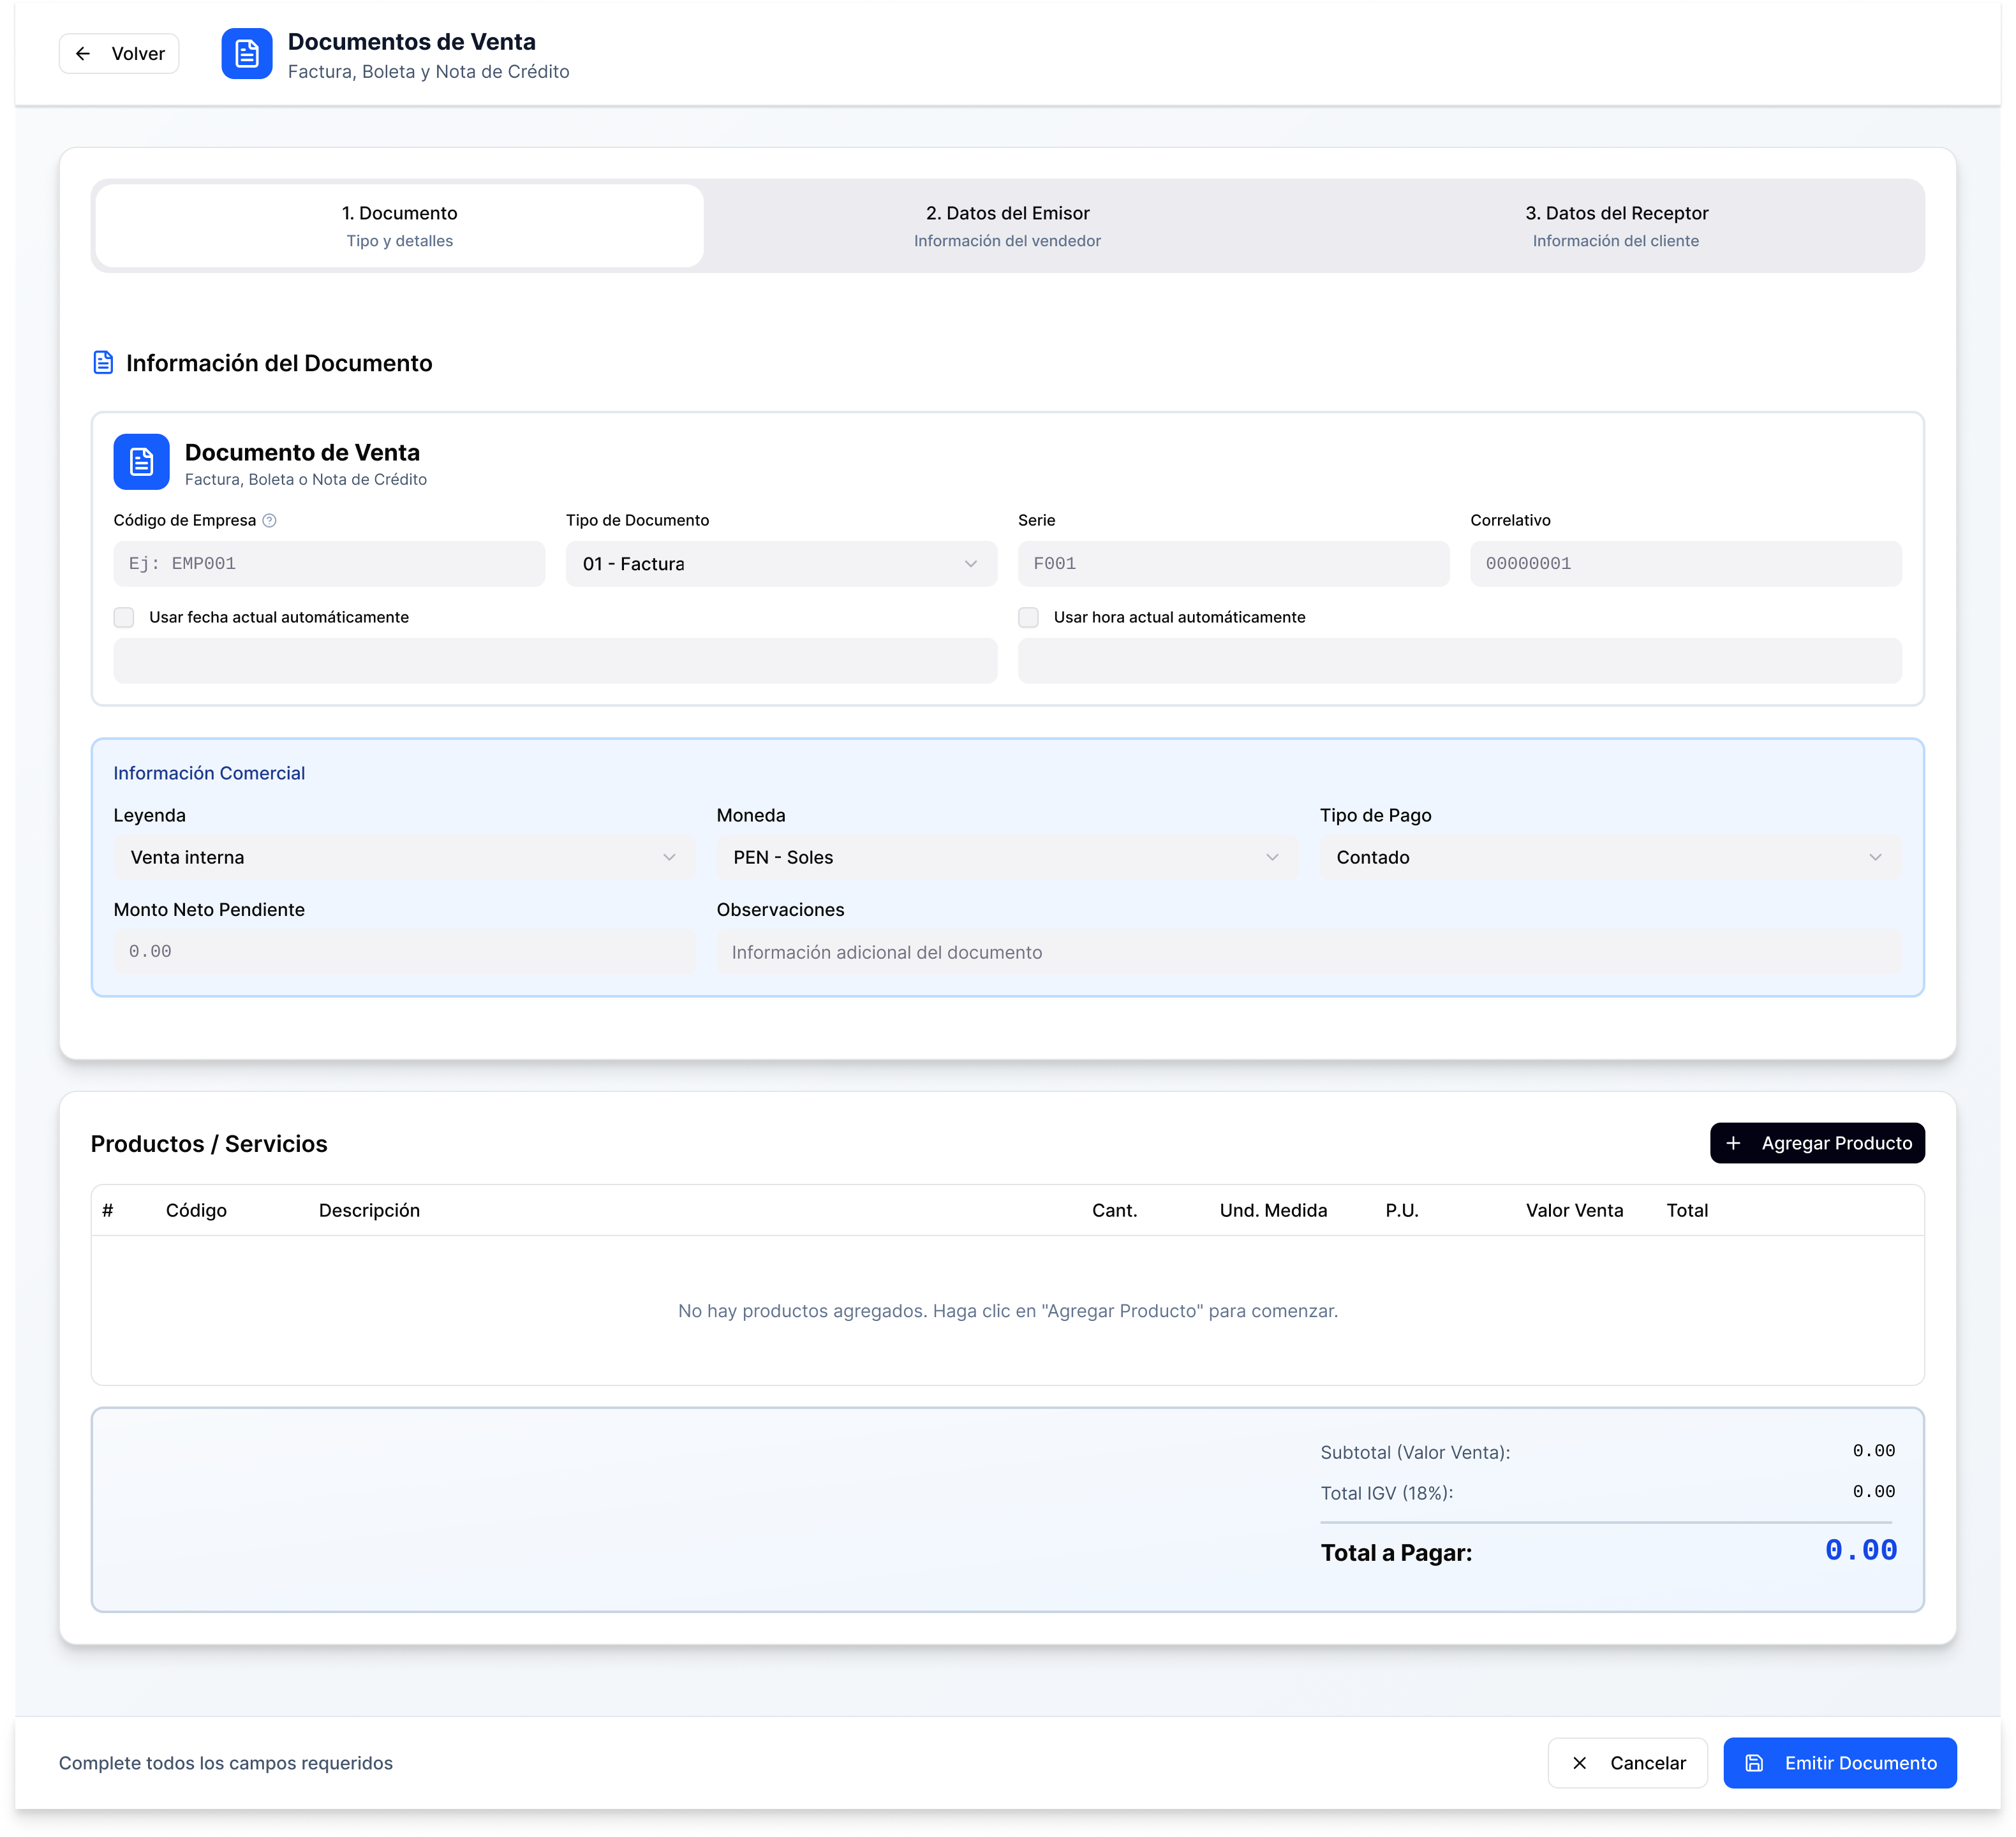
\includegraphics[width=0.9\textwidth]{Datos_Documento_Venta.png}
  \caption[Mockup de los datos del documento de venta]{Mockup de los datos del documento de venta.
  Este diseño presenta la información requerida para el registro y actualización de datos del documento de venta.}
  \label{fig:mockup-documento-venta}
\end{figure}
\newpage
\begin{figure}[htbp]
  \centering
  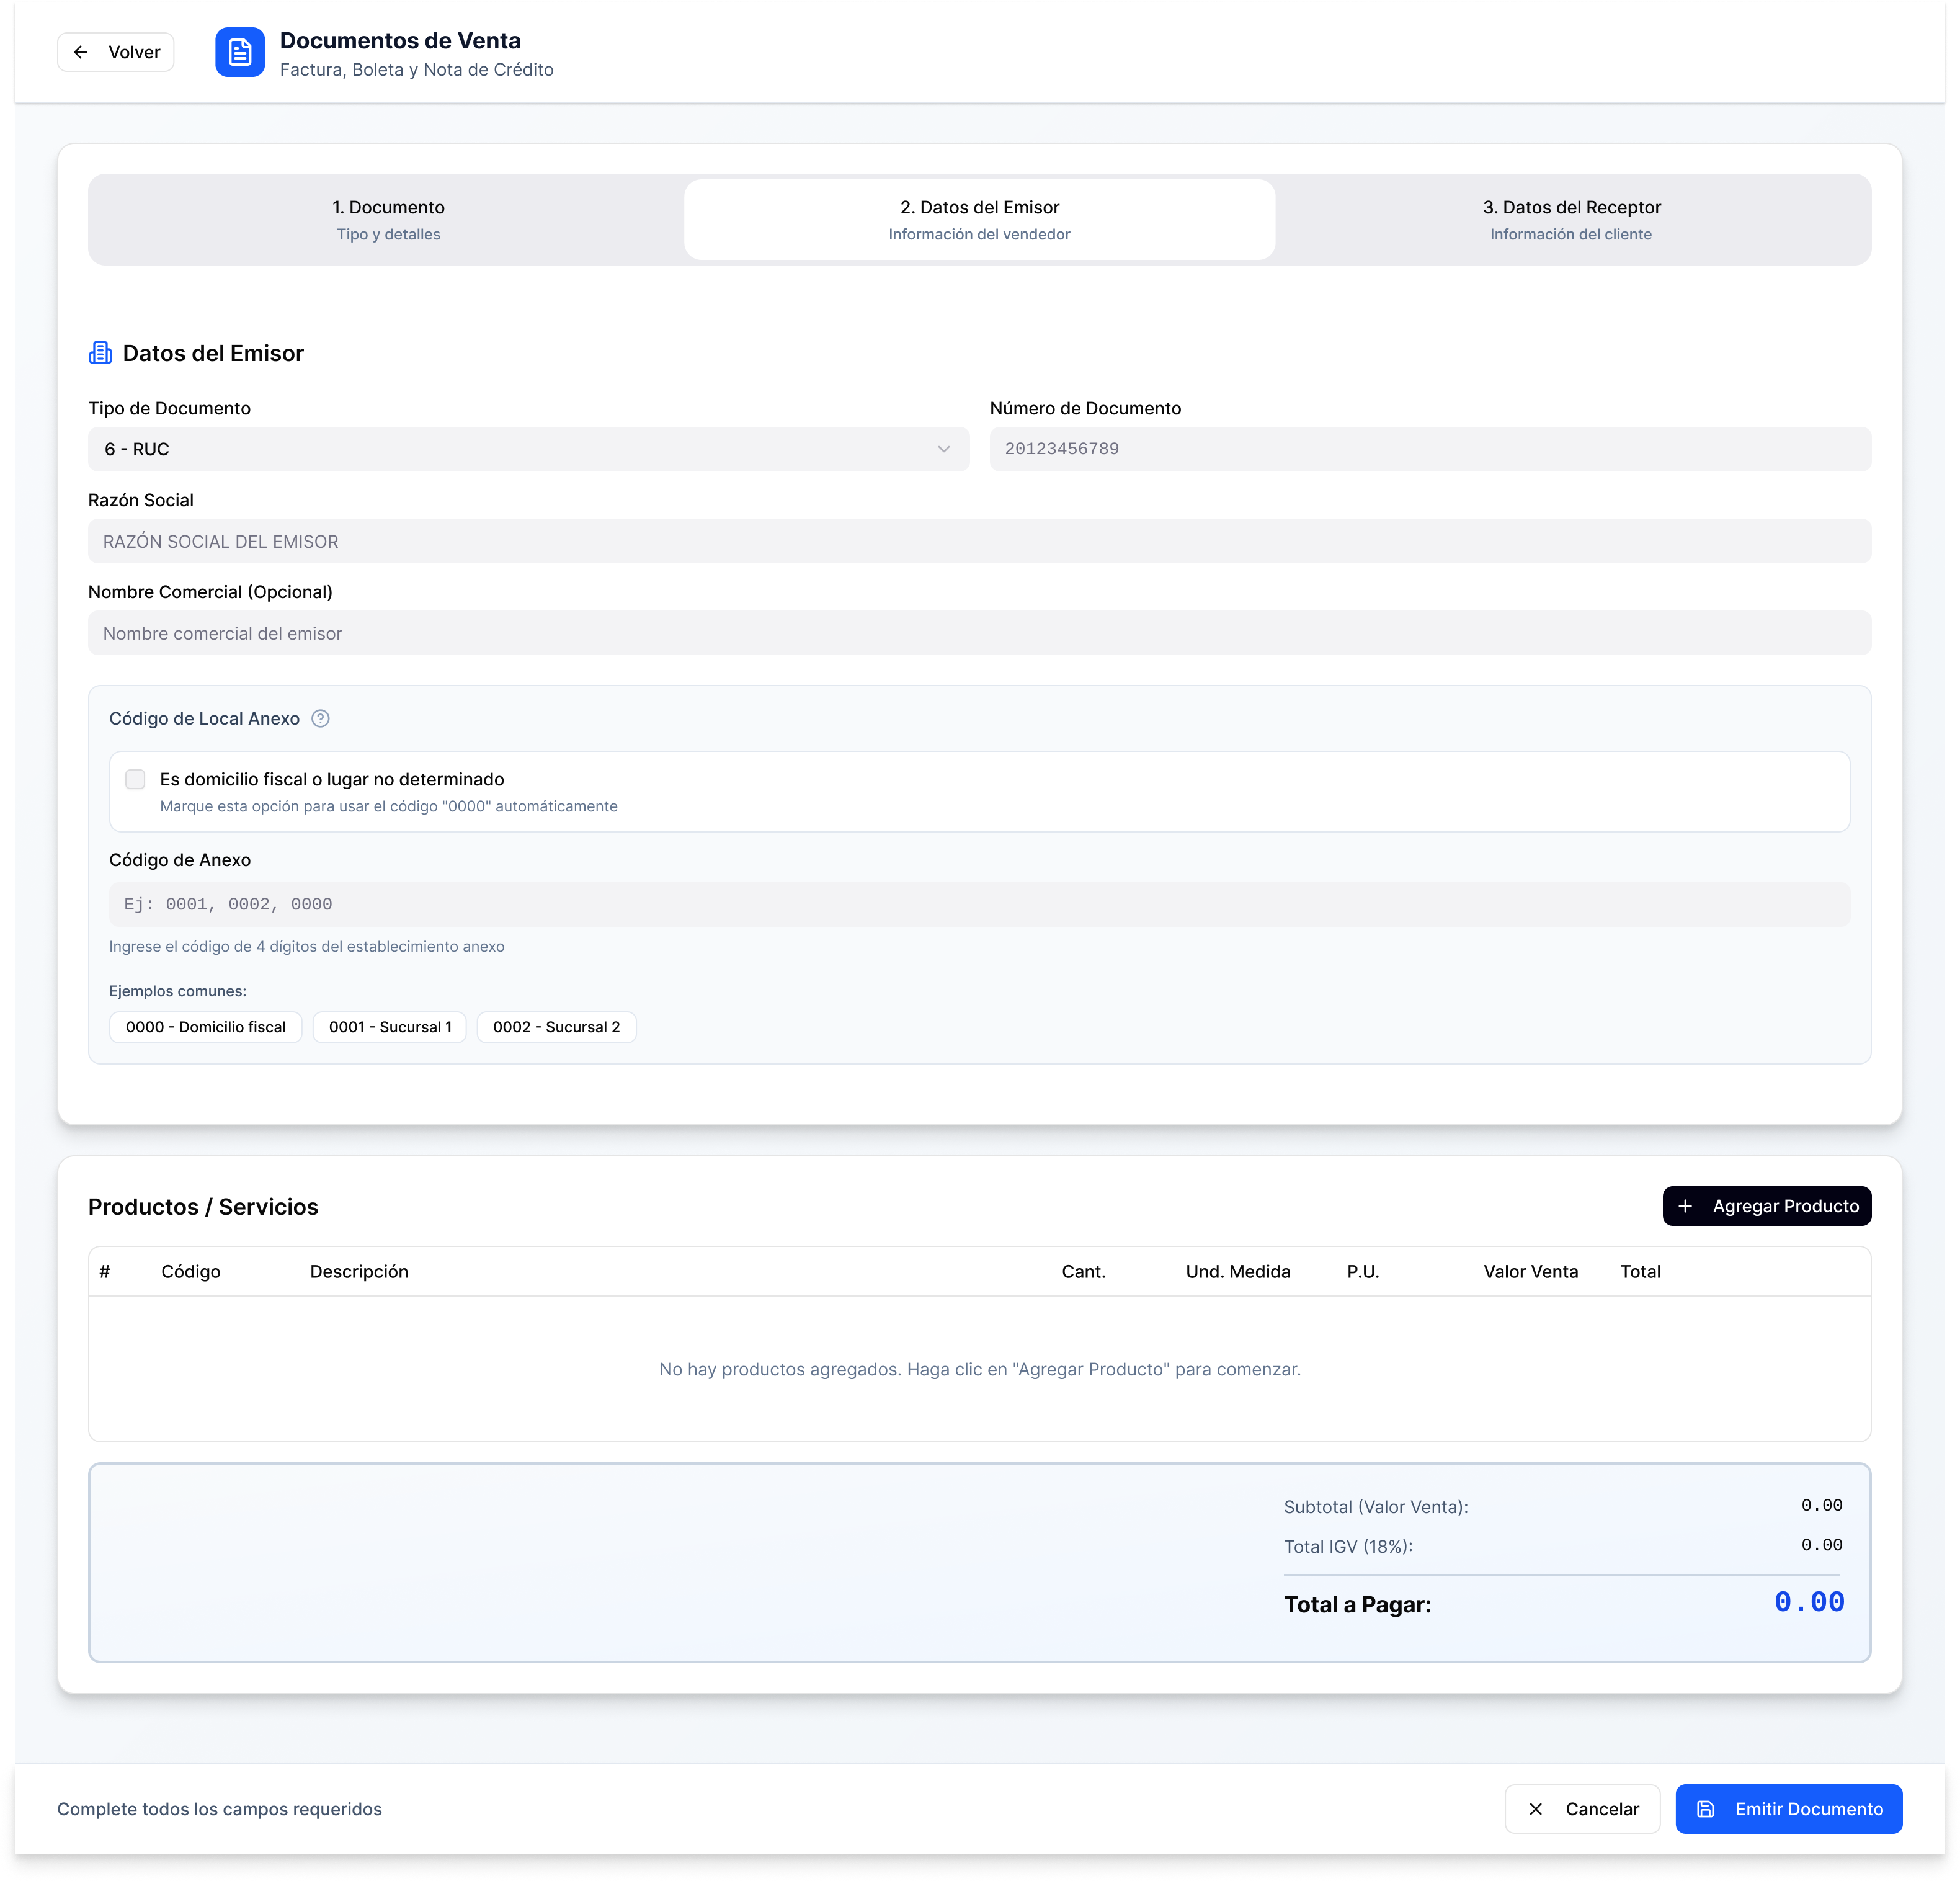
\includegraphics[width=0.9\textwidth]{Datos_Emisor.png}
  \caption[Mockup de los datos del emisor]{Mockup de los datos del emisor.
  Este diseño presenta la información requerida para el registro y actualización de datos del emisor.}
  \label{fig:mockup-emisor}
\end{figure}
\newpage
\begin{figure}[htbp]
  \centering
  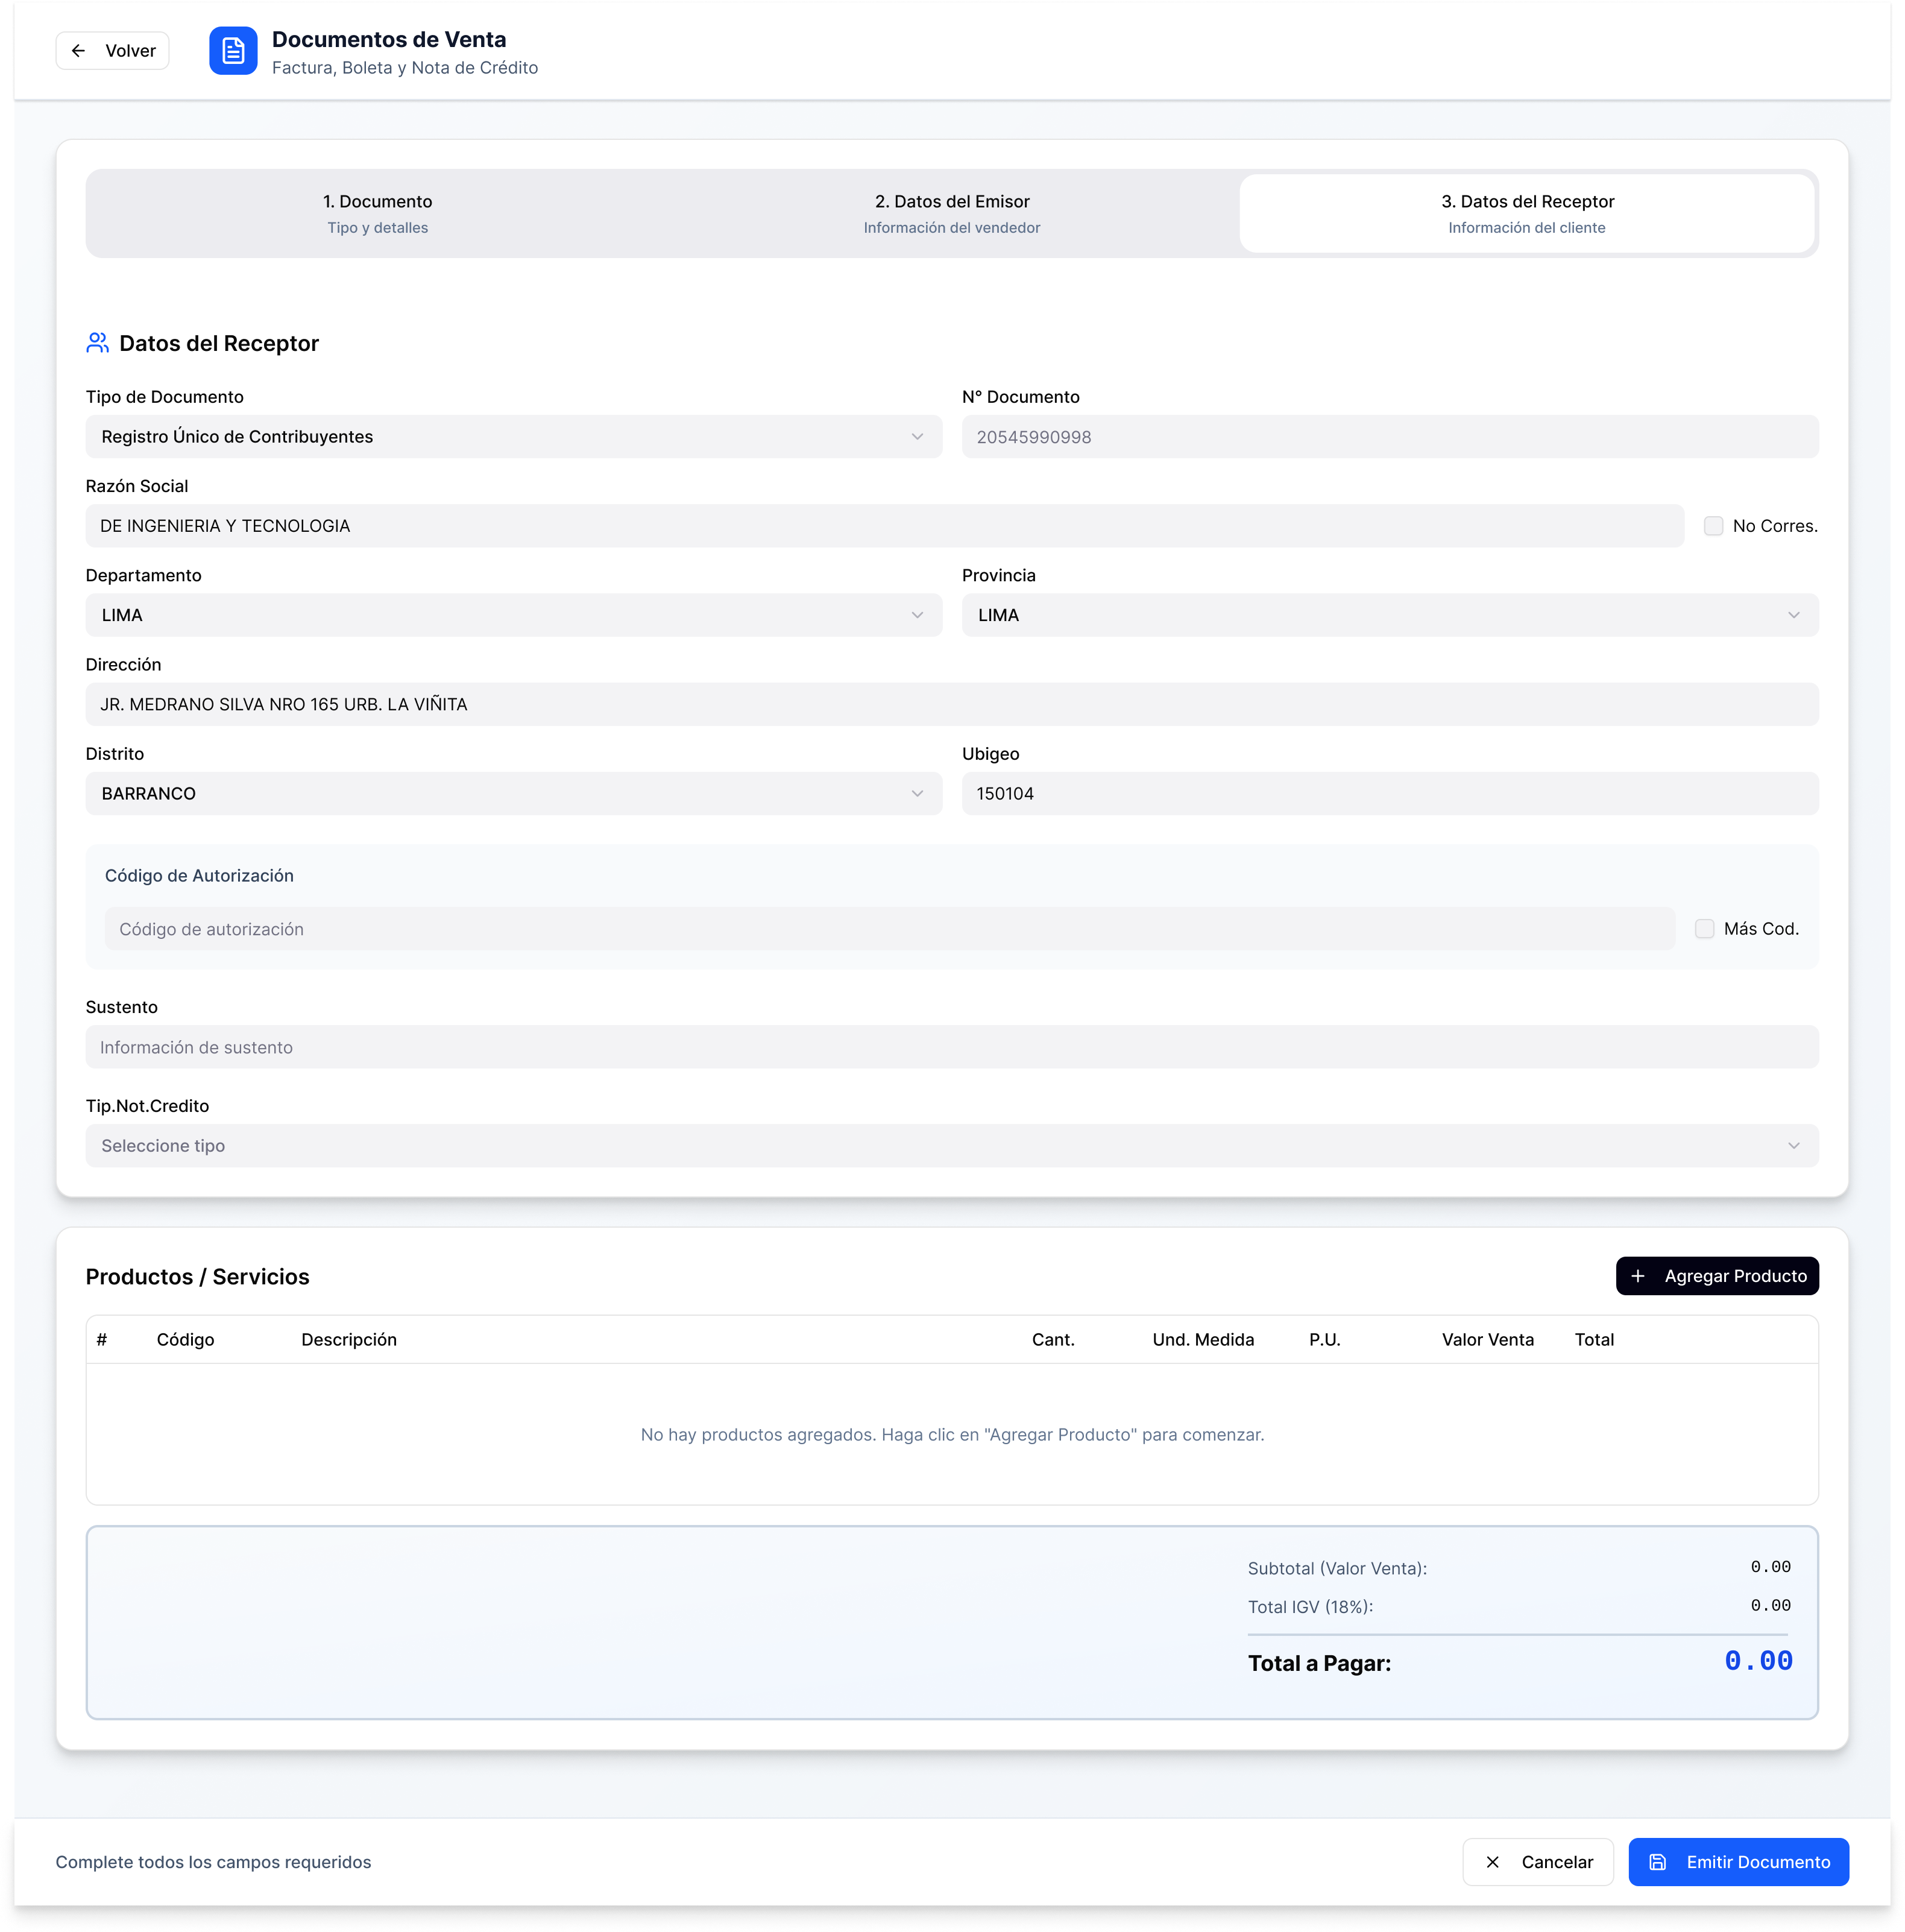
\includegraphics[width=0.9\textwidth]{Datos_Receptor.png}
  \caption[Mockup de los datos del receptor]{Mockup de los datos del receptor.
  Este diseño presenta la información requerida para el registro y actualización de datos del receptor.}
  \label{fig:mockup-receptor}
\end{figure}
\newpage
\begin{figure}[htbp]
  \centering
  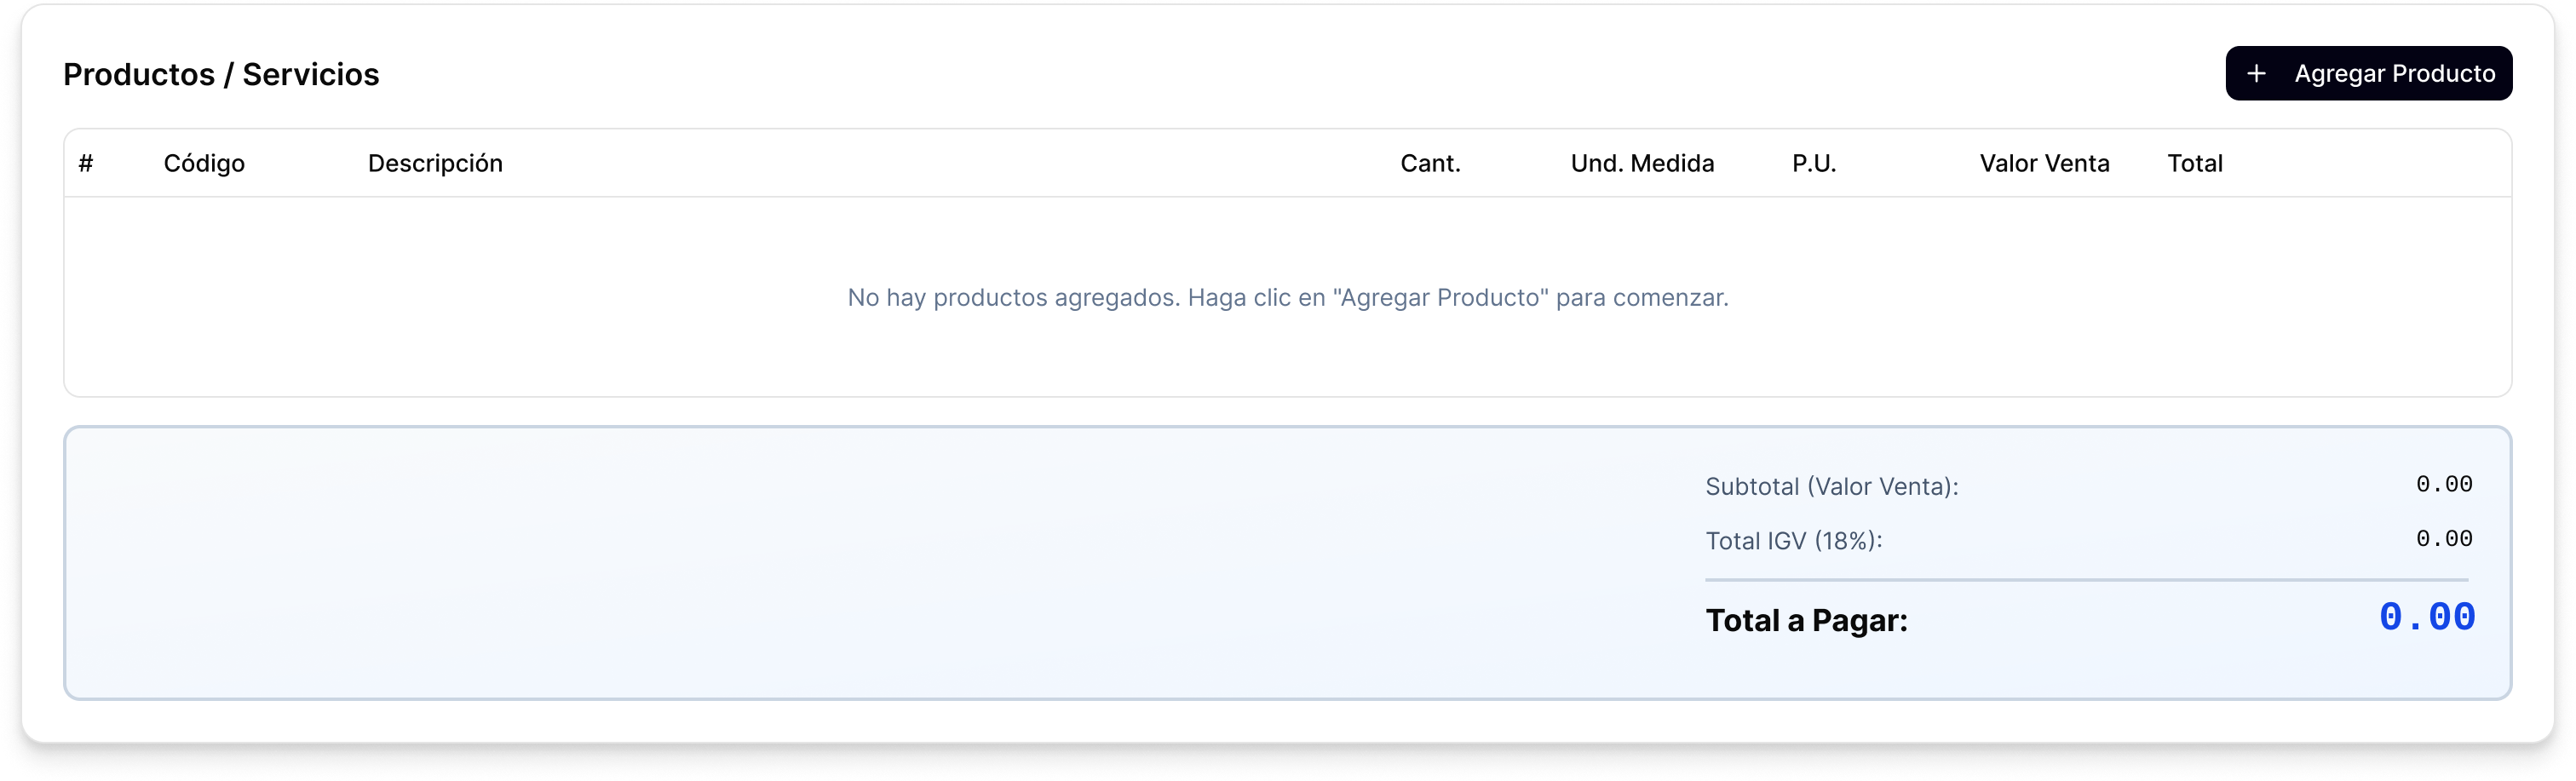
\includegraphics[width=0.9\textwidth]{Datos_Productos.png}
  \caption[Mockup de los datos del producto]{Mockup de los datos del producto.
  Este diseño presenta la información requerida para el registro y actualización de datos del producto.}
  \label{fig:mockup-producto}
\end{figure}

\section{Organización del equipo}
El equipo de desarrollo está conformado por seis integrantes, organizados según roles específicos que permiten una adecuada distribución de responsabilidades y un flujo de trabajo ordenado. La siguiente tabla detalla los roles asignados y sus funciones principales.

\begin{table}[htbp]
  \caption[Organización del equipo]{Organización del equipo: roles y responsabilidades principales.}
  \label{tab:organizacion-equipo}
  \centering
  \singlespacing
  \setlength{\tabcolsep}{4pt}
  \renewcommand{\arraystretch}{1.15}
  \begin{tabularx}{\textwidth}{@{}L{0.20\textwidth} L{0.22\textwidth} Y@{}}
    \toprule
    Integrante & Rol & Responsabilidades principales \\
    \midrule
    Integrante 1 & Líder de proyecto & Coordinación general, planificación, seguimiento del avance, comunicación con el docente. \\
    Integrante 2 & Analista funcional & Levantamiento de requisitos, modelado de procesos, validación con el cliente. \\
    Integrante 3 & Arquitecto de software & Diseño de la estructura del sistema, definición de componentes y estándares técnicos. \\
    Integrante 4 & Desarrollador backend & Implementación de lógica del sistema, APIs, validaciones y manejo de datos. \\
    Integrante 5 & Desarrollador frontend & Construcción de interfaces, integración con backend, experiencia de usuario. \\
    Integrante 6 & Tester / QA & Elaboración de casos de prueba, verificación funcional, reporte de errores. \\
    \bottomrule
  \end{tabularx}
\end{table}

\section{Gestión del control de versiones (Git)}
Para garantizar un desarrollo ordenado, trazable y colaborativo, el proyecto emplea Git como sistema de control de versiones, siguiendo un flujo basado en ramas que permite separar las etapas de desarrollo, integración y corrección de errores. La organización de ramas se establece de la siguiente manera:

\subsection{Ramas del proyecto}
\begin{itemize}
  \item \texttt{main}: Es la rama principal y contiene las versiones estables y listas para producción del proyecto. Solo se integran cambios previamente probados y validados.
  \item \texttt{develop}: Rama destinada al desarrollo continuo. En ella se integran las funcionalidades provenientes de las ramas \texttt{feature/*} antes de ser preparadas para una futura liberación.
  \item \texttt{feature/*}: Ramas dedicadas a la creación de funcionalidades específicas. Cada característica nueva debe desarrollarse dentro de una rama separada del tipo \texttt{feature/\allowbreak nombre-funcionalidad}. Una vez completada, se fusiona con la rama \texttt{develop}.
  \item \texttt{hotfix/*}: Ramas utilizadas para corregir errores críticos en la rama \texttt{main}. Permiten atender incidencias urgentes sin interferir con el flujo de desarrollo. Tras corregirse el problema, los cambios se integran tanto en \texttt{main} como en \texttt{develop}.
\end{itemize}

\subsection{Normas de normalización de commits}
Para mantener un historial claro, uniforme y fácil de interpretar, se empleará una convención basada en el estándar Conventional Commits. Cada mensaje debe iniciar con un prefijo que indique el tipo de cambio realizado.

\subsubsection{Estructura de un commit}
\texttt{tipo:\allowbreak descripci\'on breve y clara en infinitivo}

\subsubsection{Tipos de commits permitidos}
\begin{itemize}
  \item \texttt{feat:} Se utiliza para incorporar una nueva funcionalidad o módulo al sistema. Ejemplo: \texttt{feat:\allowbreak agregar generaci\'on de XML UBL para factura}.
  \item \texttt{fix:} Usado para corregir errores o incidencias del sistema. Ejemplo: \texttt{fix:\allowbreak corregir error en validaci\'on de RUC emisor}.
  \item \texttt{docs:} Para modificaciones en documentación (manuales, comentarios, diagramas). Ejemplo: \texttt{docs:\allowbreak actualizar descripci\'on del m\'odulo de gu\'ias}.
  \item \texttt{style:} Ajustes que no afectan la lógica del código, como formato, identación o renombrado menor. Ejemplo: \texttt{style:\allowbreak ajustar formato de clases en servicio XML}.
  \item \texttt{refactor:} Cambios en el código que mejoran su estructura interna sin alterar su comportamiento. Ejemplo: \texttt{refactor:\allowbreak optimizar m\'etodo de construcci\'on de nodos XML}.
  \item \texttt{test:} Para agregar o modificar pruebas automatizadas. Ejemplo: \texttt{test:\allowbreak a\~nadir pruebas para m\'odulo de notas de cr\'edito}.
  \item \texttt{chore:} Tareas menores o de mantenimiento que no afectan directamente el producto final, como actualización de dependencias. Ejemplo: \texttt{chore:\allowbreak actualizar librer\'ias de generaci\'on de PDF}.
\end{itemize}

\subsubsection{Reglas adicionales}
\begin{itemize}
  \item La descripción debe ser corta y clara, escrita en infinitivo.
  \item Evitar mensajes genéricos como ``cambios'', ``arreglos'' o ``update''.
  \item Cada commit debe representar un cambio coherente y aislado.
  \item Antes de hacer un commit, verificar que el código compila y no rompe funcionalidades existentes.
\end{itemize}


\section{Desarrollo de la primera fase (login)}
La primera fase del proyecto consistió en la implementación del módulo de autenticación de usuarios, el cual constituye la puerta de acceso al sistema. Esta etapa tuvo como objetivo garantizar que únicamente usuarios registrados y autorizados puedan ingresar a la plataforma.

Para ello, se desarrolló una interfaz de inicio de sesión simple, funcional y orientada a la usabilidad. El formulario incluye los campos de correo electrónico y contraseña, además de validaciones básicas en el lado del cliente para evitar el envío de datos incompletos. Asimismo, se implementaron mensajes de error claros cuando las credenciales no coinciden o cuando se detectan campos vacíos.

En el lado del servidor, se configuró el endpoint correspondiente para recibir las credenciales y validarlas contra la base de datos. Las contraseñas almacenadas se encuentran cifradas utilizando algoritmos seguros, lo que garantiza la protección de la información sensible. Una vez verificada la autenticidad de los datos ingresados, el sistema genera un token de acceso y redirige al usuario hacia el panel principal de acuerdo con su rol.

Finalmente, se consolidó la documentación técnica del módulo, describiendo el flujo de proceso, los endpoints involucrados, los códigos de error generados y las consideraciones de seguridad aplicadas. Esta base garantiza la extensibilidad del sistema para incluir futuras funcionalidades como recuperación de contraseña, registro de nuevos usuarios o autenticación de dos factores.
\section{Documentación del repositorio}
El repositorio del proyecto ha sido organizado y documentado siguiendo lineamientos que permiten asegurar claridad estructural, coherencia técnica y una colaboración eficiente entre los integrantes del equipo. Para ello, se elaboró un archivo principal \texttt{README.md}, el cual describe los aspectos fundamentales del sistema, incluyendo el stack de tecnologías utilizadas, la estructura de ramas del control de versiones, los pasos para la ejecución del proyecto, las funcionalidades actualmente disponibles y un apartado de evidencias que respalda el avance del desarrollo.

El repositorio se encuentra dividido en dos módulos principales: Frontend y Backend, cada uno con su respectivo archivo \texttt{README.md} destinado a explicar su estructura interna, dependencias, instrucciones de despliegue y convenciones particulares.

En el módulo Frontend, desarrollado con React y TypeScript, se incorpora documentación interna mediante JSDoc. Esto permite detallar componentes, propiedades, funciones y flujos esenciales, garantizando mantenibilidad y facilitando la incorporación de nuevos desarrolladores. Por su parte, el módulo Backend, construido con Java y Spring Boot, utiliza JavaDoc para describir controladores, servicios, entidades y procesos asociados. Adicionalmente, el backend cuenta con una documentación interactiva generada mediante Swagger UI, donde se expone de forma clara y navegable cada endpoint de la API, sus parámetros, modelos de datos y respuestas esperadas. Esta herramienta contribuye a la validación, prueba y comprensión del comportamiento de los servicios implementados.

El repositorio también integra los lineamientos formales para el uso de Git. Se adopta un flujo basado en las ramas \texttt{main}, \texttt{develop}, \texttt{feature/} y \texttt{hotfix/}, permitiendo un desarrollo ordenado, controlado y rastreable. A ello se suma una convención estandarizada para los mensajes de commit, orientada a mantener un historial claro y uniforme.

En conjunto, la documentación del repositorio proporciona una base sólida para la mantenibilidad del sistema, permite que cualquier integrante pueda comprender rápidamente su estructura y garantiza la continuidad del desarrollo en fases posteriores.

\section{Conclusiones }
% ── REFERENCIAS ─────────────────────────────────────────
\newpage
\nocite{*}
\printbibliography[title={Referencias}]

\end{document}